%2369
\newpage
\subsection{キーボードで絵を動かしてみよう}

スクリプトエディタの、ファイル→「開く」メニューから「move.hsp」を読み込んで実行してみてください。


\begin{figure}[H]
    \begin{center}
      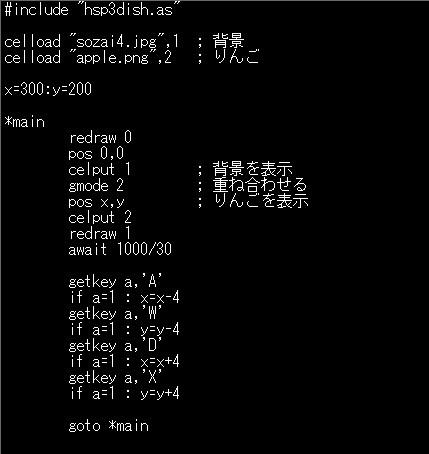
\includegraphics[keepaspectratio,width=10.61cm,height=11.229cm]{text04-img/text04-img037.png}
      \caption{move.hspの実行画面}
    \end{center}
    \label{fig:prog_menu}
\end{figure}

これは背景とりんごを表示するプログラムですが、リンゴを「A」「W」「D」「X」のキーを押して動かすことができます。何だかゲームみたいですね。

りんごをどのように動かしているのでしょうか。

いままでは、「x=x+2」のような行を入れて、1コマずつ動かしていました。

今度は、キーボードのボタンを押している時だけ、動くようにすればいいのです。

そのために、以前にも使った条件判断の仕組みを利用します。

キーボードが押されているかどうかを条件判断するために、新しい命令、getkeyの使い方を覚えておきましょう。

\begin{description}
    \item \textgt{\bf \ \ getkey 変数 , ‘キーの文字’}
\end{description}

と書くことで、指定した変数にキーが押されたかどうかが数値として代入されます。

たとえば、


\begin{description}
    \item \textgt{\bf \ \ getkey a, ‘X’}
\end{description}


を実行すると、「X」キーの状態で変数aの値が0か1になります。


\begin{description}
    \item \textgt{\bf 「X」のキーが押されていない時は、変数aは0になります。}
    \item \textgt{\bf 「X」のキーが押されている時は、変数aは1になります。}
\end{description}

キーの文字は、必ず大文字で’A’のように書く必要があるので注意してください。

文字の代わりにキーコードと呼ばれる数字を指定することで、特殊なキーの状態を知ることもできます。


\begin{description}
    \item \textgt{\bf \ \ キーコード : 実際のキー}
    \item \textgt{\bf \ {}-{}-{}-{}-{}-{}-{}-{}-{}-{}-{}-{}-{}-{}-{}-{}-{}-{}-{}-{}-{}-{}-{}-{}-{}-{}-{}-{}-{}-{}-{}-{}-{}-{}-{}-{}-{}-{}-{}-{}-{}-{}-   }
    \item \textgt{\bf \ \ \ \ \ \ \ \ 1 \ \ \ : マウスの左ボタン}
    \item \textgt{\bf \ \ \ \ \ \ \ \ 2 \ \ \ : マウスの右ボタン}
    \item \textgt{\bf \ \ \ \ \ \ \ \ 8 \ \ \ : [BACKSPACE]}
    \item \textgt{\bf \ \ \ \ \ \ \ \ 9 \ \ \ : [TAB]}
    \item \textgt{\bf \ \ \ \ \ \ \ 13 \ \ \ : [ENTER]}
    \item \textgt{\bf \ \ \ \ \ \ \ 16 \ \ \ : [SHIFT]}
    \item \textgt{\bf \ \ \ \ \ \ \ 17 \ \ \ : [CTRL]}
    \item \textgt{\bf \ \ \ \ \ \ \ 18 \ \ \ : [ALT]}
    \item \textgt{\bf \ \ \ \ \ \ \ 32 \ \ \ : スペースキー}
    \item \textgt{\bf \ \ \ \ \ \ \ 37 \ \ \ : カーソルキー[←]}
    \item \textgt{\bf \ \ \ \ \ \ \ 38 \ \ \ : カーソルキー[↑]}
    \item \textgt{\bf \ \ \ \ \ \ \ 39 \ \ \ : カーソルキー[→]}
    \item \textgt{\bf \ \ \ \ \ \ \ 40 \ \ \ : カーソルキー[↓]}
    \item \textgt{\bf \ \ \ 48〜57 \ \ \ : [0]〜[9](メインキーボード)}
    \item \textgt{\bf \ \ \ 65〜90 \ \ \ : [A]〜[Z]}
    \item \textgt{\bf \ \ 96〜105 \ \ \ : [0]〜[9](テンキー)}
    \item \textgt{\bf \ 112〜121 \ \ \ : ファンクションキー [F1]〜[F10]}
\end{description}

こうして代入された0か1の値を条件判断によって、やりたい内容を書くことで色々なことに応用ができます。

%2491
